\subsubsection{Consulta e avaliação de uma entrega}
\label{ssub:entrega_avaliacao}

Ao carregar numa entrega, o utilizador é direcionado para uma página onde pode consultar as informações da referida entrega, assim como proceder à sua avaliação.\\

Nesta página o utilizador pode consultar a descrição da entrega, fazer download dos ficheiros que a constituem e consultar os resultados dos testes a que a entrega foi submetida.\\

Pode também facilmente avaliar os alunos que constituem o grupo que efetuou a entrega, indicando a sua avaliação e uma nota auxiliar.\\

Na Figura~\ref{fig:delivery_grades} pode ser consultada uma imagem demonstrativa da página desenvolvida.

\begin{figure}[H]
  \centering
  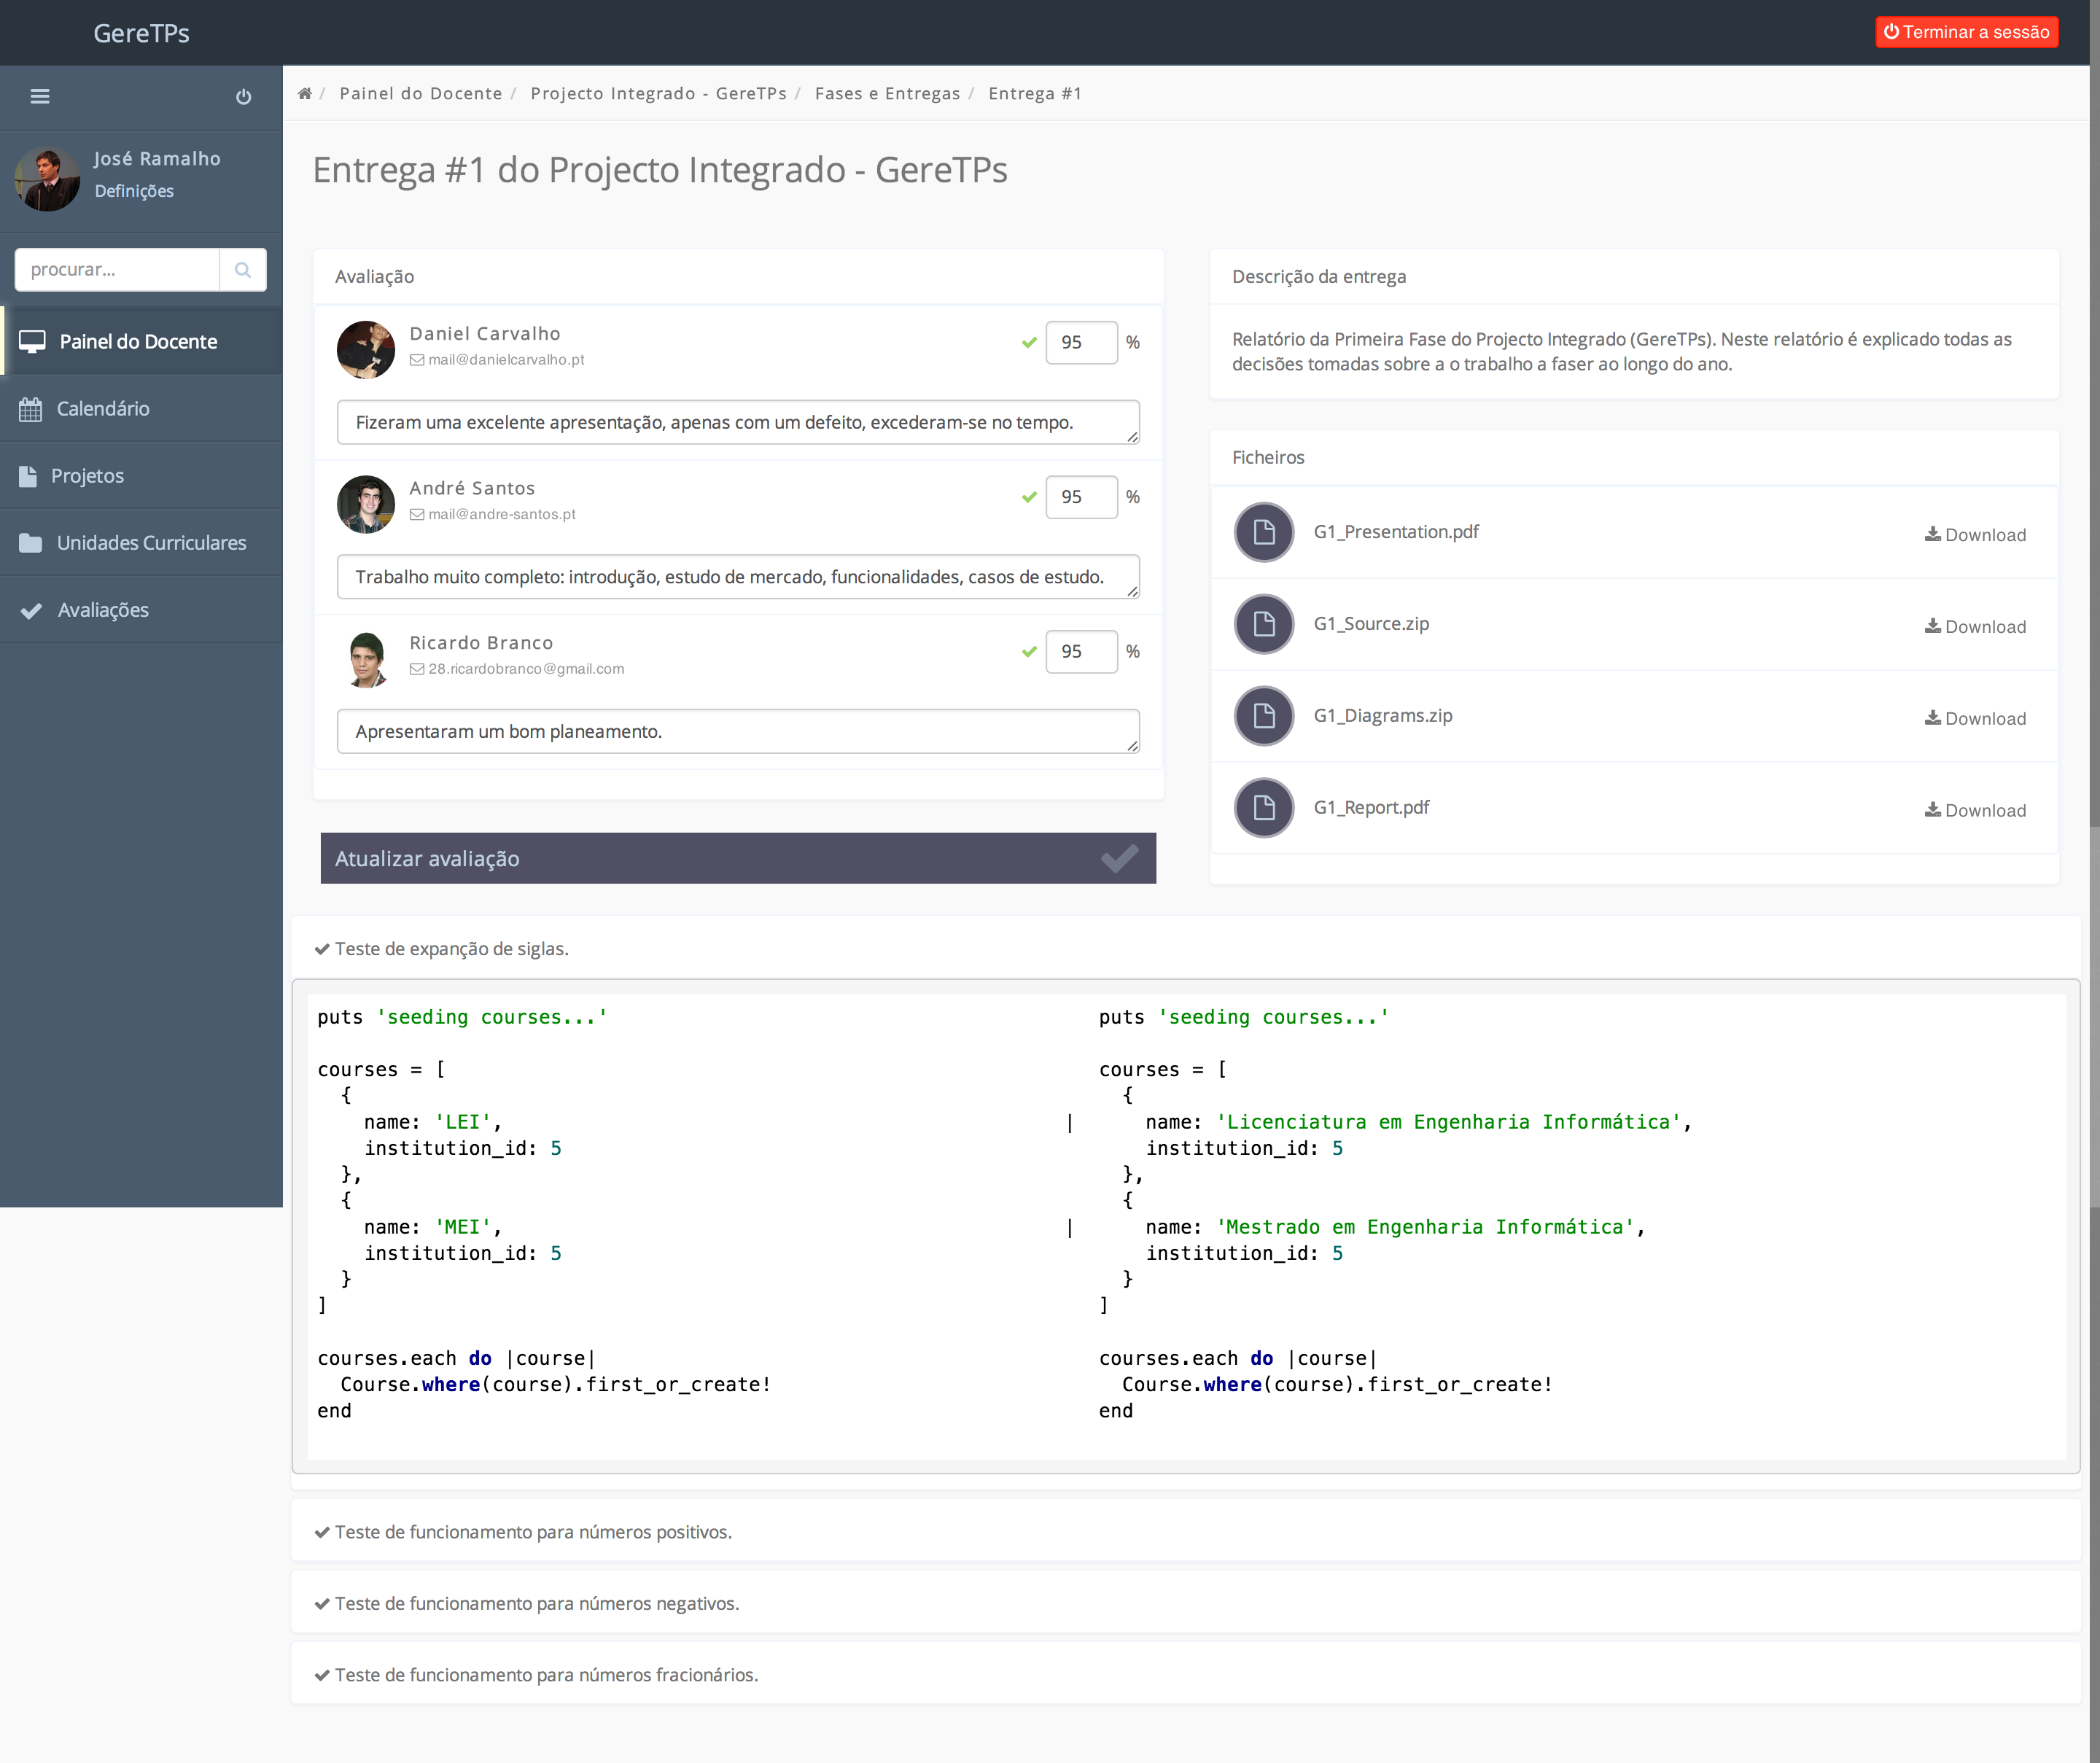
\includegraphics[width=1\textwidth,center]{images/implementacao/docentes/delivery_and_grades}
  \caption{Página de consulta e avaliação de uma entrega}
  \label{fig:delivery_grades}
\end{figure}
